\clearpage
\section{Metodologia}

Największy nacisk w trakcie tworzenia pracy został położony na łatwość wdrożenia. 
W poniższych podrozdziałach przedstawiono kwestie, które należy wziąć pod uwagę
podczas projektowania rozwiązania, które ma tę cechę spełniać.

\subsection{Architektura systemu}

Wśród możliwych architektur systemów można wyłonić dwie najważniejsze gałęzie: 
architektura monolityczna lub oparta na mikroserwisach, które są małymi, niezależnymi 
od siebie aplikacjami, wspólnie ze sobą współpracującymi. Pierwsza z opcji opiera się 
na idei polegającej na tym, że wszelka funkcjonalność danego systemu jest zamknięta 
w jednym projekcie i funkcjonuje jako całość. Druga możliwość opiera się na 
rozdzieleniu funkcjonalności na wiele mniejszych podprogramów, które działają 
niezależnie od siebie. Obydwie architektury posiadają swoje wady i zalety i wybór 
jednej z nich zależy od specyficznych potrzeb każdego projektu. W tabeli 
\ref{tab:porownanie-architektur}. przedstawiono porównanie obydwu architektur 
\cite{newmanb2015}, które 
uwzględnia:

\begin{itemize} % lista nienumerowana
    \item Odporność systemu na awarie. System powinien być w każdym momencie dostępny 
    dla użytkowników
    \item Skalowalność. Potrzeba skalowania wynika ze zbyt dużego obciążenia dla jednego 
    lub większej ilości serwisów w jednostce czasu. Brak dopasowania zasobów do 
    aktualnego zapotrzebowania może prowadzić do tego, że system nie będzie odpowiadał 
    na żądania użytkowników
    \item Łatwość wdrożenia. Architektura systemu nie powinna utrudniać wdrożenia nowych 
    funkcjonalności
    \item Zespół deweloperski. Architektura systemu nie powinna wymagać zatrudnienia 
    wielu programistów
\end{itemize}

    \begin{xltabular}{1\textwidth} { 
        | >{\raggedright\arraybackslash}X 
        | >{\centering\arraybackslash}X 
        | >{\raggedleft\arraybackslash}X | }
        \caption{Porównanie popularnych architektur systemów} \label{tab:porownanie-architektur} \\
        \hline
       Cecha & System monolityczny & System oparty na architekturze mikroserwisowej \\
        \hline
       Odporność systemu na awarie & 
       W przypadku awarii w jednym punkcie, cały system przestaje działać & 
       awaria jednego z serwisów niekoniecznie musi oznaczać niesprawność całego systemu \\
       \hline
       Skalowalność & 
       Wymusza zwiększanie liczby instancji wszystkich usług, nawet jeśli zapotrzebowanie 
       na część z nich jest małe & 
       Możliwość zwiększania liczby instancji tylko tych usług, które w danym momencie są 
       silnie obciążone \\
      \hline
      Łatwość wdrożenia &
      Nawet mała zmiana w kodzie aplikacji monolitycznej wymaga ponownego wdrożenia całego 
      kodu &
      Możliwość szybkiego wdrożenia poprawek w obrębie danego mikroserwisu \\
      \hline
      Zespół deweloperski &
      Rozbudowany projekt zazwyczaj wymaga zespołu liczącego setki programistów, co 
      utrudnia komunikację i zmniejsza efektywność pracy &
      Nie wymaga rozbudowanego zespołu, możliwość oddelegowania małej grupy pracowników 
      do oddzielnych mikroserwisów \\
      \hline
    \end{xltabular}

Biorąc pod uwagę zestawienie z tabeli \ref{tab:porownanie-architektur}. Postanowiono wykorzystać architekturę 
mikrousługową w celu implementacji systemu.

\subsubsection{Serwisy zorientowane usługowo}

Docelowo, system oparty na architekturze mikrousługowej powinien składać się z serwisów 
zorientowanych usługowo (ang. \textit{service-oriented architecture}). Stanowią one 
konstrukcję, w której wiele serwisów współpracuje ze sobą w celu zapewnienia zbioru 
funkcjonalności. Serwis oznacza tutaj oddzielny proces pracujący na danej maszynie. 
Procesy te komunikują się ze sobą przez sieć.

\subsubsection{Sprzężenie serwisów}

Architektura mikrousługowa opiera się na tym, że poszczególne serwisy działają 
niezależnie od siebie. Dzięki temu zmiany wprowadzone w jednym serwisie nie powinny 
wymagać zmian w drugim. Ponadto wdrożenie danego serwisu nie powinno wymagać 
jednoczesnego wdrożenia innych. O tak rozdzielonych serwisach mówi się, że są ze sobą 
luźno sprzężone (ang. \textit{loose coupling}). Prawidłowo skonstruowany serwis powinien 
wiedzieć jedynie tyle, w jaki sposób może komunikować się z innymi serwisami w celu 
uzyskania wymaganych danych.

\subsubsection{Spójność serwisów}
W prawidłowo skonstruowanym systemie mikrousługowym funkcjonalność związana ze 
sobą (np. w kontekście biznesowym) jest umieszczona w jednym miejscu. O tak 
zaprojektowanych serwisach mówi się, że są one spójne (ang. \textit{high cohesion}). 
Przykładem 
błędnej implementacji może być edycja danych osobowych klienta w wielu serwisach. 
Wtedy zmiana w jednym serwisie może wymagać zmiany w innych.

\subsubsection{Architektura systemu do zarządzania energią w pomieszczeniach biurowych}

Opierając się na poprzednich podrozdziałach oraz w oparciu o założenia utworzono 
architekturę systemu będącego rezultatem tej pracy inżynierskiej. Rysunek 
\ref{fig:architektura-systemu} przedstawia pełną architekturę aplikacji:

\begin{figure}[h]
    \centering
    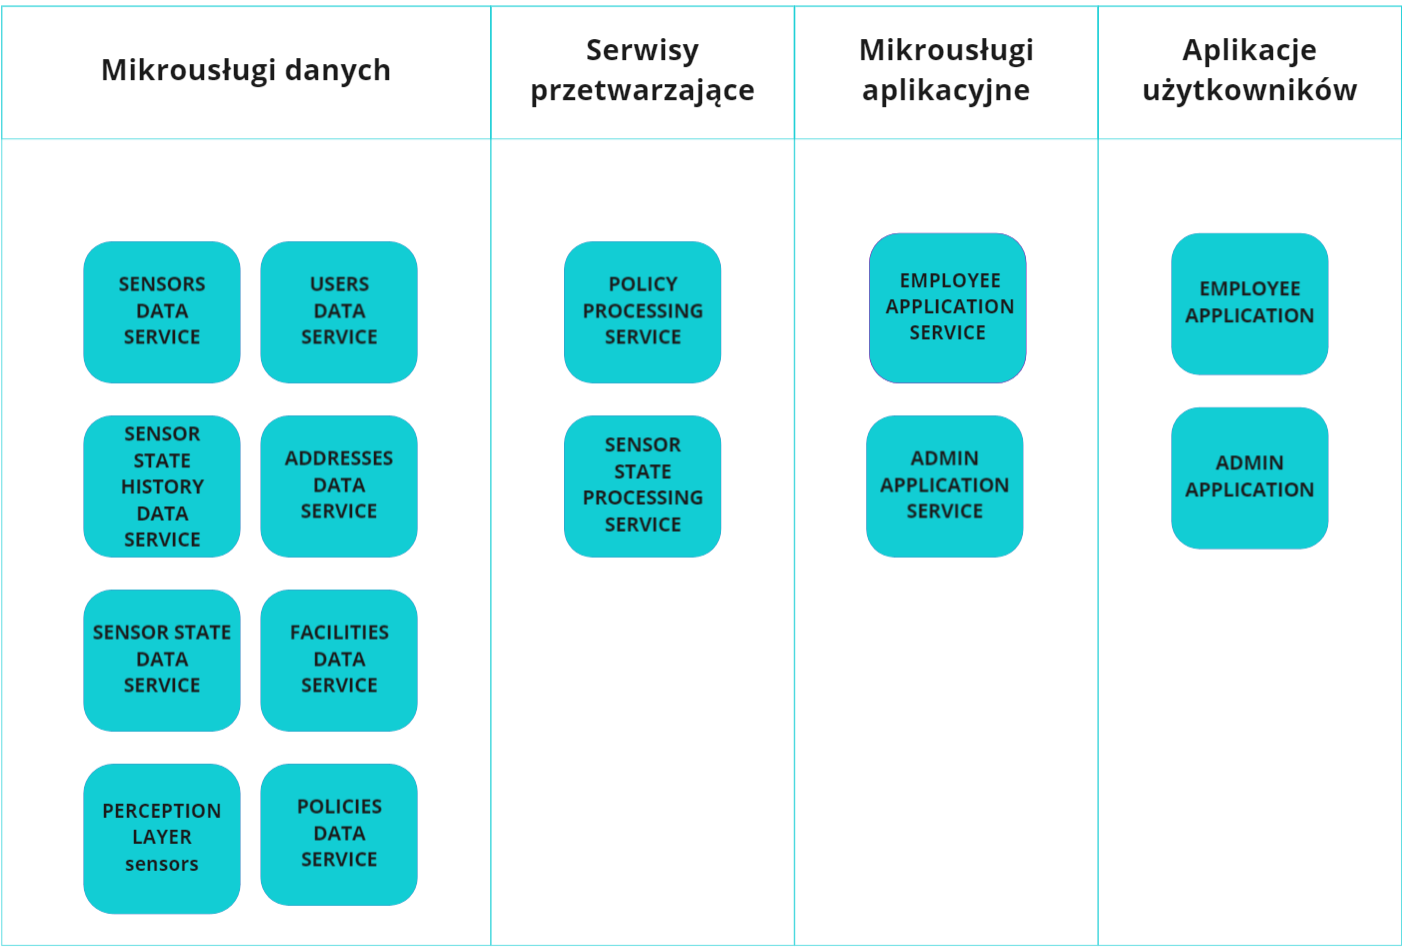
\includegraphics[width=1\textwidth]{architektura.jpg}
    \caption{Architektura systemu}
    \label{fig:architektura-systemu}
\end{figure}

Na całość składają się serwisy opisane w tabeli \ref{tab:mikrouslugi-danych}.

    \begin{xltabular}{1\textwidth} { 
        | >{\raggedright\arraybackslash}X        
        | >{\raggedright\arraybackslash}X | }
        \caption{Mikrousługi danych} \label{tab:mikrouslugi-danych} \\
        \hline
       Nazwa & Funkcja \\
       \hline
       Addresses data service & 
       Przechowuje adresy organizacji oraz poszczególnych budynków \\
       \hline
       Facilities data service &
       Przechowuje szczegółowe dane dotyczące budynków \\
       \hline
       Policies data service & 
       Przechowuje reguły określające oczekiwaną wartość mierzonych parametrów \\
       \hline
       Sensors data service &
       Przechowuje szczegółowe dane dotyczące wykorzystywanych czujników \\
       \hline
       Sensor state history data service &
       Przechowuje historyczne pomiary z poszczególnych czujników \\
       \hline
       Sensor state data service &
       Przesyła pomiary od czujników \\
       \hline
    \end{xltabular}

Poza mikrousługami danych aplikacja posiada również serwisy przetwarzające dane:

    \begin{xltabular}{1\textwidth} { 
        | >{\raggedright\arraybackslash}X        
        | >{\raggedright\arraybackslash}X | }
        \caption{Serwisy przetwarzające} \label{tab:serwisy-przetwarzajace} \\
        \hline
       Nazwa & Funkcja \\
       \hline
       Sensor state processing service & 
       Otrzymuje dane z czujników. Zajmuje się ich prawidłowym zapisaniem, po czym wysyła 
       je dalej do serwisu sprawdzającego zgodność wyników rzeczywistych z oczekiwanymi \\
       \hline
       Policy processing service &
       Przetwarza dane z czujników. Porównuje pomiary rzeczywiste z oczekiwanymi, które 
       zostały określone w regułach \\
       \hline
    \end{xltabular}

Na system składają się także mikrousługi aplikacyjne:

    \begin{xltabular}{1\textwidth} { 
        | >{\raggedright\arraybackslash}X        
        | >{\raggedright\arraybackslash}X | }
        \caption{Mikrousługi aplikacyjne} \label{tab:mikrouslugi-aplikacyjne} \\
        \hline
       Nazwa & Funkcja \\
       \hline
       Employee application service & 
       Usługa aplikacyjna dla aplikacji pracowników. Oferuje styki umożliwiające 
       zarządzanie kontem, tworzenie własnych reguł dla pomieszczeń przypisanych do 
       konkretnego użytkownika oraz sprawdzanie ich aktualnego stanu \\
       \hline
       Admin application service &
       Usługa aplikacyjna dla aplikacji administratorów. Oferuje wszystkie styki 
       udostępniane pracownikom, a ponadto styki umożliwiające zarządzanie informacjami 
       dotyczącymi organizacji, budynków, pomieszczeń i czujników \\
       \hline
    \end{xltabular}

Ostatnimi elementami systemu są aplikacje dla poszczególnych ról użytkowników:

    \begin{xltabular}{1\textwidth} { 
        | >{\raggedright\arraybackslash}X        
        | >{\raggedright\arraybackslash}X | }
        \caption{Aplikacje użytkowników} \label{tab:aplikacje-uzytkownikow} \\
        \hline
       Nazwa & Funkcja \\
       \hline
       Employee application & 
       Oferuje graficzny interfejs do interakcji z usługą aplikacyjną pracowników \\
       \hline
       Admin application &
       Oferuje graficzny interfejs do interakcji z usługą aplikacyjną administratorów \\
       \hline
    \end{xltabular}